\chapter{Photon Detection System}
\label{ch:fdsp-pd}
\fixme{\color{blue} Chapter editor: Wilson}
%
%%
%%%%%%%%%%%%%%%%%%%%%%%%%%%%%%%%%%%%%%%%%%%%%%%%%%%%%%%%%%%%%%%%%%%%

\section{Photon Detection System (PD) Overview}
\label{sec:fdsp-pd-ov}
%\fixme{(Length: TDR=10 pages, TP=3 pages)}
\metainfo{(Length: TDR=10 pages, TP=3 pages)}

%%%%%%%%%%%%%%%%%%%%%%%%%%%%%%%%%
\subsection{Introduction}
\label{sec:fdsp-pd-intro}
\fixme{\color{blue} Content: Segreto}
TEST WITH ANNE
The Photon Detection System provides ...

\fixme{In the TP introduction there should be a statement concerning the photon collector options under consideration and the timeline and procedure for making a selection.}

The system includes (whatever it includes), as shown in Figure.... 

\fixme{Include an image of the overall system, indicating its parts. Show how the system fits into the overall detector.}

The operating principle is illustrated in Figure~\ref{figure-label}... (add figure)

\begin{dunefigure}[optional caption for LoF]{fig:figure-label}
{required full caption (Credit: xyz)}
%\includegraphics[width=0.8\textwidth]{image-filename}
\end{dunefigure}

\fixme{Include summary of simulation status? {\color{red}  Szelc/Himmel}}

%%%%%%%%%%%%%%%%%%%%%%%%%%%%%%%%%%%%%
\subsection{Design Considerations}
\label{sec:fdsp-pd-des-consid}
\fixme{\color{blue} Content: Segreto/Warner/Mualem}

The Photon Detection system design must enable... 
...

\fixme{Anne suggests: Within this section add ref to requirements document  when it's ready, and maybe list the most important half dozen in a table here). E.g.,}  


\begin{dunetable}
[Important requirements on the PD system design]
{p{0.8\textwidth}}
{pdphysicsparams}
{Important requirements on the PD system design}   
Requirement  \\ \toprowrule
  \\ \colhline
   \\ \colhline
 ...\\ 
\end{dunetable}

\fixme{By the end of the volume, for every requirement listed in this section, there should exist an explanation of how it will be satisfied.}

\subsection{Criteria for photon collection options performance evaluation}?\fixme{\color{blue} Content: Segreto}


%%%%%%%%%%%%%%%%%%%%%%%%%%%%%%%%
\subsection{Scope}
\label{sec:fdsp-pd-scope}
\fixme{\color{blue} Content: Segreto/Warner/Mualem}

The scope of the Photon Detection system includes the continued procurement of materials for, and the fabrication, testing, delivery and installation of the following systems: 

\fixme{Whatever the items are...}

\begin{itemize}
\item Photon Collectors 
\item SiPMs
\item ...
\end{itemize}



%%%%%%%%%%%%%%%%%%%%%%%%%%%%%%%%%%%%%%%%%%%%%%%%%%%%%%%%%%%%%%%%%%%%
\section{PD Design}
\label{sec:fdsp-pd-design}
\fixme{(Length: TDR=50 pages, TP=20 pages)}
\fixme{\color{blue} Content: Conveners}

\fixme{Include an image of the subsystem, indicating its parts. Show how the system fits into the overall system).}


%%%%%%%%%%%%%%%%%%%%%%%%%%%%%%%%%%%
\subsection{Photon Collector}
\label{sec:fdsp-pd-pc}
\fixme{\color{blue} Content: Cavanna/Whittington/Machado}

At the time of the Technical Proposal there are three photon collector options  under consideration, 
in the following we summarize the design and development status for each. 
[For the Technical Design Report there will be a baseline design and an alternate.]

\subsubsection{Dip-Coated Light Guides (4 pages)}
\label{ssec:fdsp-pd-pc-bar1}
\fixme{\color{blue} Content: Toups (tbc)}

\subsubsection{Double-Shift Light Guides (4 pages)}
\label{ssec:fdsp-pd-pc-bar2}
\fixme{\color{blue} Content: Whittington}
The double-shift light guide photon collector design aims to maximize the active VUV-sensitive 
area of the photon detection system module while minimizing the necessary photocathode (SiPM) 
coverage. 
Commercially-fabricated plastic can be manufactured to transport light via total internal 
reflection with low attenuation losses. However, direct application of coatings to such
 manufactured optical surfaces can have an adverse impact on the effective attenuation length 
by introducing or exaggerating imperfections in the surface quality. 
To maintain the long intrinsic attenuation length of a manufactured light guide, the 
double-shift light guide design decouples the conversion of VUV photons to optical by
 arraying acrylic plates coated with TPB in front of a commercially-fabricated polystyrene 
light guide doped with a second wavelength-shifting compound.

\paragraph*{Description}

Figure~\ref{fig:DoubleShiftLG-Cartoon} illustrates the process by which LAr scintillation 
photons are converted and detected by a double-shift light guide module. VUV scintillation
 photons impinging on the acrylic plates are converted to blue wavelengths. A portion of
 these blue photons penetrate the light guide and are converted to green. The isotropic 
re-emission of these green photons leads to a significant fraction becoming trapped by 
total internal reflection within the light guide. Trapped photons are transported to 
the end of the light guide where they are detected by an array of SiPMs.

\begin{figure}[ht]
  \begin{center}
%  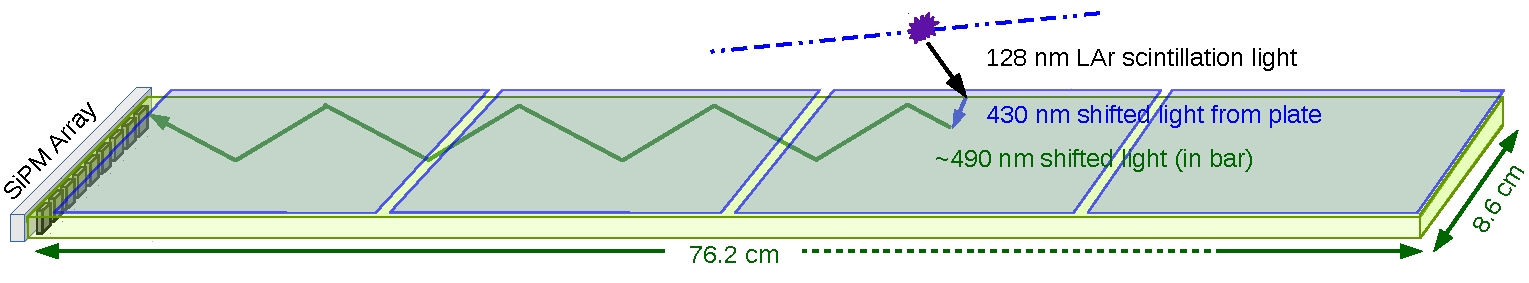
\includegraphics[width=0.9\columnwidth]{DoubleShiftLG-Cartoon.pdf}
  \caption{Cartoon schematic of the operation of a double-shift light guide.}\label{fig:DoubleShiftLG-Cartoon}
  \end{center}
\end{figure}

\paragraph*{Wavelength-Shifting Plates}

Acrylic spray-coated with TPB. TPB absorption and emission properties.

\paragraph*{Wavelength-Shifting Light Guide}

EJ-280 light guides manufactured by Eljen Technologies\footnote{http://www.eljentechnology.com}. 
EJ-280 absorption and emission properties. PDE of SiPMs.

\paragraph*{Testing}

The double-shift light guide design has undergone a series of development 
iterations to improve its performance, carried out at Indiana University and at 
Fermi National Laboratory's cryogenic and vacuum test facility (PAB). 
Comparative testing of light guide designs at PAB in mid-2015 demonstrated 
the double-shift light guide concept~\cite{bib:JINST-11-C05019}.
 An improved design similar to that deployed at ProtoDUNE-SP was studied at 
the Blanche test stand at Fermilab in September of 2016 with a complementary 
component-wise analyis program at Indiana University afterward, detailed in 
Ref.~\cite{bib:DoubleShiftLG-NIM-171113}. The attenuation characteristics of 
this light guide were measured at Indiana University, while the global quantum 
efficiency for detecting incident LAr scintillation photons was measured with 
a vacuum-ultraviolet monochromator at Indiana University and using 
scintillation light from cosmic rays at the Blanche test stand.

\paragraph*{Performance}

Analysis of the double-shift light guide's attenuation properties determined 
an attenuation profile in LAr characterized by a double-exponential function
 of the form $f(z) = A \exp(-z/\lambda_{A}) + B \exp(-z/\lambda_B)$ with $z$ 
the distance from the instrumented end and parameters $A = $0.29,
 $\lambda_A = $4.3cm, $B = $0.71, and $\lambda_B = $225 cm~\cite{bib:DoubleShiftLG-NIM-171113}. 
The effective attenuation length is comparable to the width of an APA 
when the double-shift light guide is deployed in liquid argon.

Using both approaches the global quantum efficiency of this detector was 
determined to be 0.48\% at the readout end. Combined with the attenuation 
function and integrated over the area of the module dimensions planned for
 the DUNE far detector, this corresponds to an effective area for detecting
 VUV scintillation photons of 3.7 cm$^{2}$ per module. Wavelength-shifting 
plates are deployed on both sides of the light guide, meaning the double-shift
 light guide modules in the center APA array are sensitive to scintillation 
light from two drift volumes and modules in the outer arrays are able to detect
 scintillation light originating outside of the TPC volume.

Simulated response of this module within the DUNE single-phase far detector module 
indicates this module efficiency should result in an average efficiency for the 
photon detection system to detect light from neutrino interactions from a galactic 
supernova of between 30\% at 5~MeV and 70\% at 15~MeV of visible energy.

\paragraph*{Potential Improvements for the DUNE Far Detector}

The double-shift light guide deployed in the ProtoDUNE-SP APAs was constrained 
to readout at a single end. Proposed changes to the APA size and cabling routing 
scheme for the DUNE single-phase far detector would allow for a second array of 
SiPMs at the opposite end of the light guide. This would double the performance of
 the photon detection system, raising the per-module effective area to 7.4 cm$^{2}$ 
per module per drift volume.

An SiPM with a wavelength-dependent PDE that is better matched to the EJ-280 emission 
spectrum would improve the overall efficiency. Simulations of the transport of light 
within the light guide suggest that applying a highly reflective coating to the long, 
narrow inactive sides of the light guide would further boost the attenuation function
 and further increase effective area of the light guide module. These effects combined 
lead to a potential increase of the effective area to 15 cm$^{2}$ per module per drift volume.

The simulated supernova neutrino detection capability of a photon detection system 
based on this module depends strongly on small changes in the estimated efficiency.
 The potential improvements described above raise the physics performance in this 
channel into a regime where small fluctuations in the module efficiency have a 
smaller impact on the efficiency to detect these supernova neutrino interactions. 
These improvements are an important component to risk mitigation in the photon 
detection system performance.


\subsubsection{ARAPUCA (4 pages)}
\label{ssec:fdsp-pd-pc-arapuca}
\fixme{\color{blue} Content: Cavanna (?)}

\subsubsection{Hybrid or New Options (2 pages)}
\label{ssec:fdsp-pd-pc-new}

\subsection{New Techniques to Supplement or Enhance Light Yield}
\label{sec:fdsp-pd-enh}
\fixme{\color{blue} Content: Cavanna/Whittington/Machado}

\subsubsection{Hybrid and New Options}

X-ARAPUCA represents the main line of development of the ARAPUCA photo-detector design aiming to further improve the collection efficiency, while retaining the same working
 principle, mechanical design and active  photo-sensitive coverage.\\
In a sense X-ARAPUCA is a hybrid solution between the ARAPUCA and the wavelength-shifting light guide bar PDS concepts, 
where photons trapped in the ARAPUCA box are shifted and transported to the readout via total internal reflection in a light guide placed inside the box.
This solution minimizes the number of reflections on the internal surfaces of the box and thus the probability of photon loss. Simulations suggest that
 this modification will lead to a rather significant increase of the collection efficiency.
 \begin{figure}[htbp]
\begin{center}
%    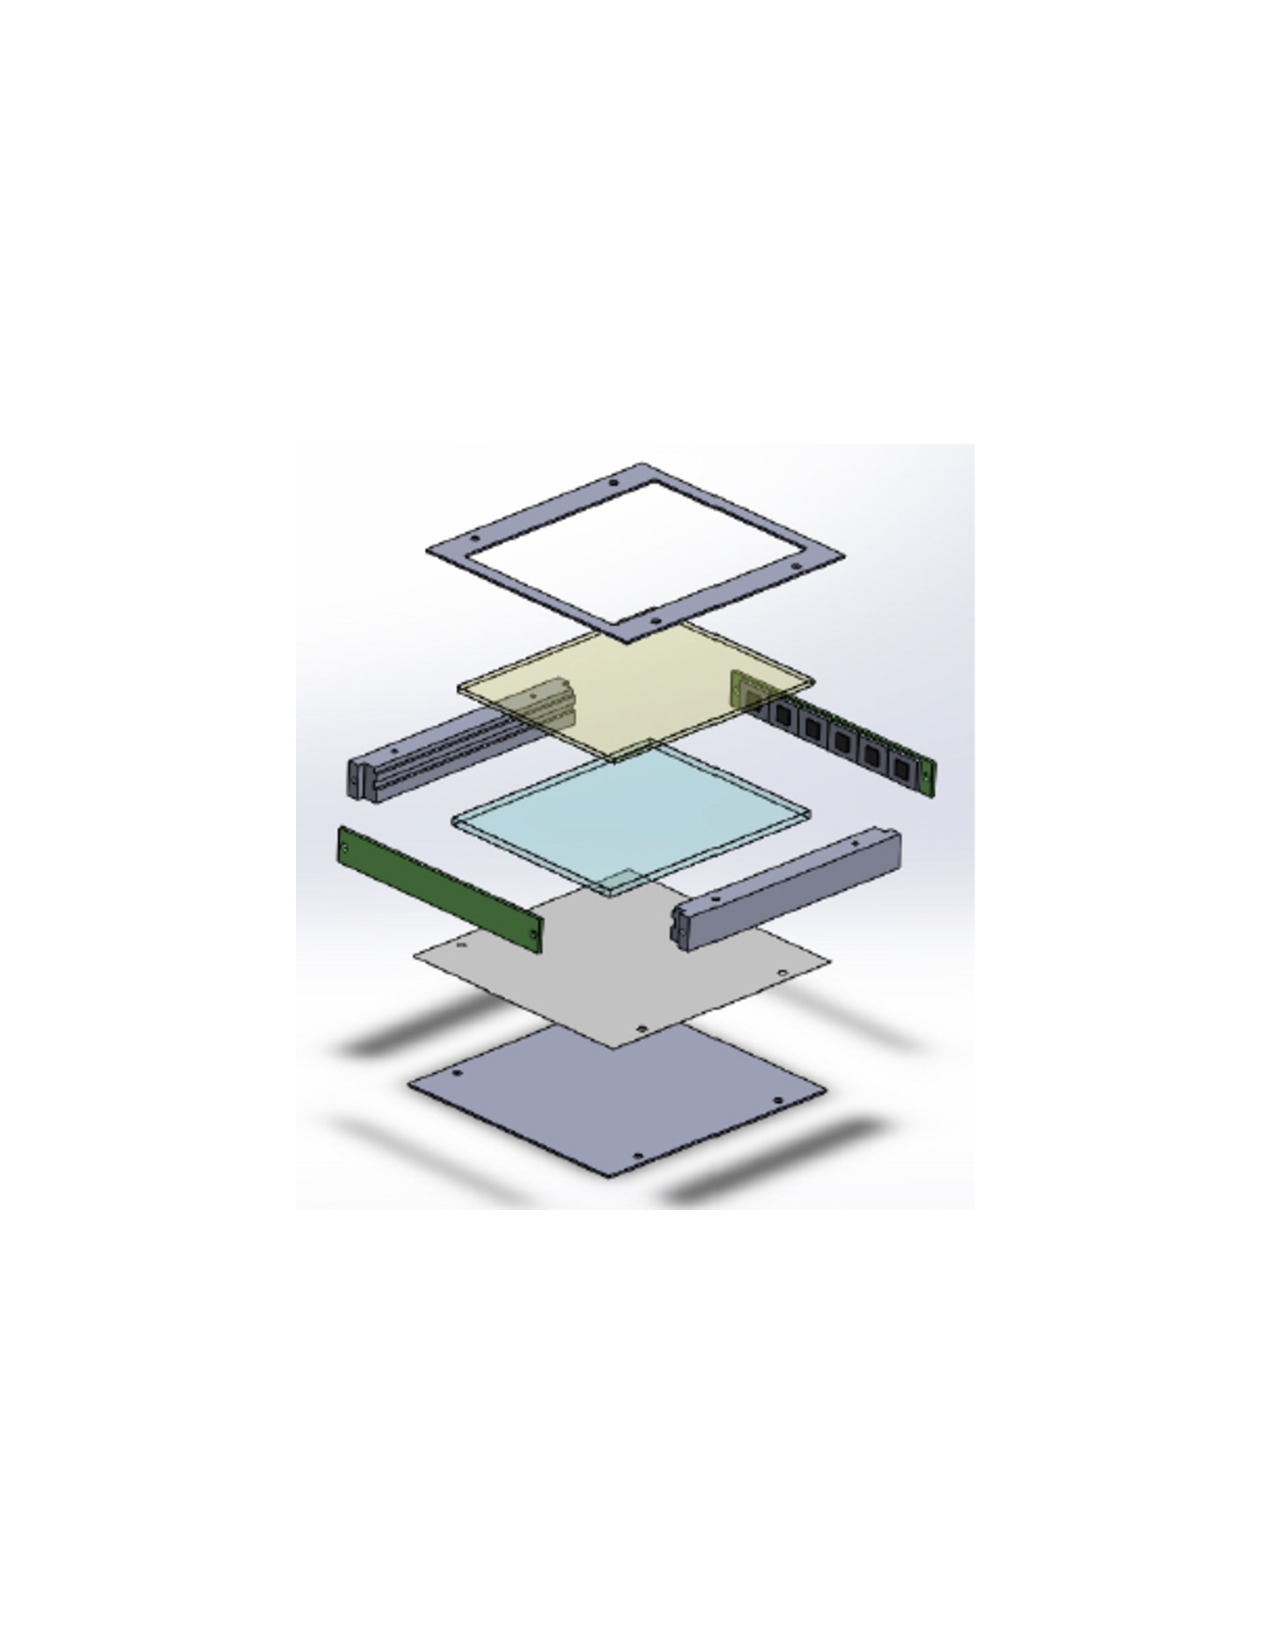
\includegraphics[height=.5\textheight]{X-Arapuca-exploded-view.pdf}
 \vspace{-2.5cm}
\caption{X-ARAPUCA design (exploded view).}
\label{fig:exploded}
\end{center}
\end{figure}

 In a standard ARAPUCA the photon trapping effect is obtained by means of a dichroic filter and a two-steps wavelength shifting process, the first from VUV to UV outside the acceptance window of the box and the second inside from UV to blue, across the filter cutoff. Double shifted photons are eventually collected by an array of photosensors (SiPM) distributed on the backplane of the box, opposite to the the acceptance window. In the X-ARAPUCA design, Fig.\ref{fig:exploded}, the inner shifter coating/lining over the reflective walls of the box is replaced by a thin wavelength-shifting light guide slab inside the box, of the same dimensions of the acceptance filter window and parallel to it. The SiPM arrays are installed vertically on the sides of the box, in optical contact to the light guide thin ends. 
 In this way a fraction of the photons will be converted inside the slab and guided to the read-out, other photons,  e.g. those at small angle of incidence below the critical angle of the light guide slab, after conversion at the slab surface will be remain trapped in the box and eventually collected as for the standard ARAPUCA.
 
 A full sized X-ARAPUCA prototype is under construction. The light guide is made by a 2 mm thick TPB doped acrylic slab. Specially designed read-out boards have been realized, made of 6 passively ganged SiPMs in a strip configuration.  Two boards into a single channel readout light signals from the X-ARAPUCA box.  \\
 
 The photon detectors described in the preceding section represent the results of a long process of optimization of the initial concepts developed years ago. A balance between the cost of the readout electronics (channel count), and the cost and performance of the SiPM's was achieved with realistic designs of the photon detectors offering the detection efficiency in the range $\sim$ 0.5 to 1.5\%.\\
A significant advances in the technology of the SPM's have been accomplished during this time: the photosensors dark count, after-pulsing and cross-talk rates have been lowered by almost an order of magnitude, whereas the production costs have been dropping significantly in response to the increasing range of applications.  The recent studies and tests demonstrate that the improved quality of the photodetectors is permitting much higher degree of ganging (passive or active), thus significantly lowering the ``per SiPM" readout costs.
These technological trends are likely to continue, thus allowing for a possible alternative concepts of the Photon Detectors, even within the geometrical and cost confines of the baseline detectors.\\
One of the possible different concepts of the Photon Detector includes a long printed circuit board with the overall dimensions identical to the light guide bars or ARAPUCA but with a simpler construction involving only SiPMs distributed over the board surface. The SiPMs can be coated with  appropriate waveshifter (TPB or MSB) or a foil with the waveshifter in front of the SiPM can be used to convert the VUV 128 nm Argon light to the blue light at the maximum detection efficiency of the SiPM. The overall detection efficiency of such a ``detector element"is expected to be of the order of 25-30\%, depending on the pixel size and the fill-factor of the SiPM.
A photon detector involving the SiPMs only would offer a major simplification of the construction and integration efforts. Its overall performance can be reliably estimated and it is proportional to the total area of the bar covered with the SiPMs.
The performance of the baseline Photon Detectors can be achieved with 2-4\% of the area covered with the SiPMs. Taking 1800 cm$^2$ as a bar surface this coverage can be accomplished with 100-200 SiPMs of the standard 6x6 mm formfactor. With 12-fold passive ganging, successfully demonstrated in recent tests, such a solution would require 8-16 readout channels per bar. The multiplexing level is limited by the noise of the readout electronics. Significantly higher degree of multiplexing can be achieved by use of larger pixel (like 75x75 microns) SiPMs and/or possible cold active ganging circuitry. 
Such a detector concept appears very flexible and it would allows for future optimization in response to the expected technological advances with no or minimal impact on the rest of the DUNE  detector. 



The Technical Proposal and TDR may include proposals to augment the capabilities of the photon
collector modules. In the case that the hardware requirements for such proposals would pose a minimal
impact on the detector design, additional R\&D beyond the timescale of the TDR may be required since it may impact the second 10~kt module if not the first. 
Some examples include:
\begin{itemize}
\item TPB-Coated Reflector Foils (Szelc)
\item Xenon-Doped LAr (Escobar/Para)
\item TPB-Doped LAr (Escobar)
\end{itemize}

%%%%%%%%%%%%%%%%%%%%%%%%%%%%%%%%%%%
\subsection{Photon Sensors}
\label{sec:fdsp-pd-ps}
\fixme{\color{blue} Content: (2 pages) - Wilson/Zutshi}
The SP DUNE Photon Detector System will use Silicon Photomultipliers, mated to
the bar or ARRAPUCA photon collector options, to detect
scintillation light generated in the LAr. Robust photon detection efficiency, low operating
voltages, small size and ruggedness make their usage entirely plausible in the single
phase design where the photon detectors are to be accommodated inside the APA 
frames. The salient guiding principles of this SiPM-based photo-detection system can be stated
as:

Signal path separate from TPC readout. This implies cables dedicated to bringing the power
in and taking the analog or digitized signals from the PD system, out of the cryostat. 
Feed-through cable space limitations therefore, imply some level of ganging of the SiPM
signals inside the LAr volume. 

The optimal SiPM may depend on the photon collector option. Since all photon collector
options being currently considered involve shifting the 128 nm LAr scintillation to 
varying degrees, the final fine-tuned choice may have to be made after the collector
downselect. It should however be kept in mind that the size of these effects, while not 
anything to sniff at, will not exceed 15-20 $\%$.

The Silicon Photomultiplier packaging should allow for tileable arrays to be constructed to
facilitate high efficiency mating to the photon collectors and efficient space utilization inside
the APA frame.

%\begin{itemize}
%\item{Silicon Photomultipliers}
%\end{itemize}

While understanding SiPM requirements (number of devices, dynamic range, triggering, 
zero-suppression threshold etc.) in light of the physics goals is an ongoing process, it is clear
from the R$\&$D carried out so far that devices from a number of vendors have the 
performance characteristics in the vicinity of that needed for the DUNE photon detector
system (see Table xxx). Furthermore, a number and types of these devices are being installed in 
proto-DUNE which will provide an excellent test bed for evaluating and monitoring SiPM
performance in a realistic environment over the medium term. 

A key requirement, based on past experience, is ensuring the mechanical and electrical 
integrity of these devices in a cryogenic environment. This is a DUNE requirement which 
catalog devices from most vendors do not satisfy as they are only certified for operation 
down to -40C. Thus it is of paramount importance for the DUNE PD Consortium to work 
with vendors in designing, fabricating and certifying SiPM packaging that is robust and
reliable from the point-of-view of long-term operation in a cryogenic environment. Already 
there is interest from atleast two vendors (Hamamatsu and FBK) to engage with the
Consortium in this fashion with the goal of having the vendor warrantying the product
for our application. Contact with other vendors and experiments (e.g. Darkside) is
being pursued.   

In parallel, comparative performance evaluation of promising SiPM candidates from
multiple vendors will need to be carried out. This evaluation will not only need to
address inherent characteristics (gain, dark rate, x-talk, after-pulsing etc) and ganging 
performance but also form factor, spectral response and mating with regard to the
multiple photon collector options. Experience acquired from proto-DUNE construction
and operation will inform QA/QC plans for the full detector which will need to be
delineated in detail.

%%%%%%%%%%%%%%%%%%%%%%%%%%
%The planned photodetector is a SiPM, model 
%SensL C-Series 6~mm$^2$
%(MicroFB-60035-SMT). % device. 
%This model of SiPM has a detection efficiency of
%41\%; the quoted detection efficiency incorporates Quantum Efficiency (QE) and 
%the effective area
%  coverage accounting for dead space between pixels.   At LAr temperature (89~K) the dark rate is of order 10~Hz
%(0.5 p.e. threshold), and  after-pulsing has not been observed. An on-going testing program is in place to ensure 
%that the SiPMs can reliably survive the stresses associated with 
%any thermal cycling in LAr and long-term operation at LAr temperature.

%All photodetectors %for ProtoDUNE-SP 
%are subjected to testing to determine
 %forward and reverse bias I-V curves,
 %breakdown voltage, dark current and dark count rate, photodetector gain, crosstalk estimation, response, and bias dependence of parameters.
 
%All SiPMs 
%Each SiPM is tested before mounting on the readout boards to determine
%if the part meets the specifications in a warm test.  After mounting to
%the readout board all items are tested both warm and cold (cyrogenic 
%temperature) to determine the operating characteristics.

%In addition to these tests, the photodetectors are tested for their
%response to light signals from an LED of appropriate wavelength.
%These tests will be sensitive enough to determine if one of the three SiPM
%elements operating in parallel is not functioning.


\fixme{rjw: Include comment whether there are differences between the photon collector options}


%%%%%%%%%%%%%%%%%%%%%%%%%%%%%%%%%%%
\subsection{Electronics}
\label{sec:fdsp-pd-pde}
\fixme{\color{blue} Content: (3 pages) - Moreno/Franchi/Djuric}

\fixme{rjw: Include comment whether there are differences between the photon collector options}

%%%%%%%%%%%%%%%%%%%%%%%%%%%%%%%%%%%
\subsection{Quality Assurance}
\label{sec:fdsp-pd-qa}
\fixme{\color{blue} Content: (1 page) - Warner}


%%%%%%%%%%%%%%%%%%%%%%%%%%%%%%%%%%%%%%%%%%%%%%%%%%%%%%%%%%%%%%%%%%%%
\section{Production and Assembly}
\label{sec:fdsp-pd-prod-assy}
\fixme{(Length: TDR=40 pages, TP=8 pages)}

%%%%%%%%%%%%%%%%%%%%%%%%%%%%%%%%%%
\subsection{Photon Collectors Production}
\label{sec:fdsp-pd-prod-pc}
\fixme{\color{blue} Content: Cavanna/Whittington/Machado}
	
\subsubsection{Dip-Coated Light Guides (2 pages)}
\label{ssec:fdsp-pd-pc-prod-bar1}

\subsubsection{Double-Shift Light Guides (2 pages)}
\label{ssec:fdsp-pd-pc-prod-bar2}

The production and assembly of the double-shift light guide modules is divided 
into separate threads for the wavelength-shifting plates and the EJ-280 light guides. 
Many of the production, quality assurance, and assembly procedures developed for the
 double-shift light guide design deployed at ProtoDUNE-SP will remain the same for 
the DUNE single-phase far detector.

\paragraph*{Manufacture of the WLS Plates}

Spray-coating of TPB on acrylic plates (see Fig.~\ref{fig:DoubleShiftLG-SprayedPlates}).

\begin{figure}[ht]
  \begin{center}
 % 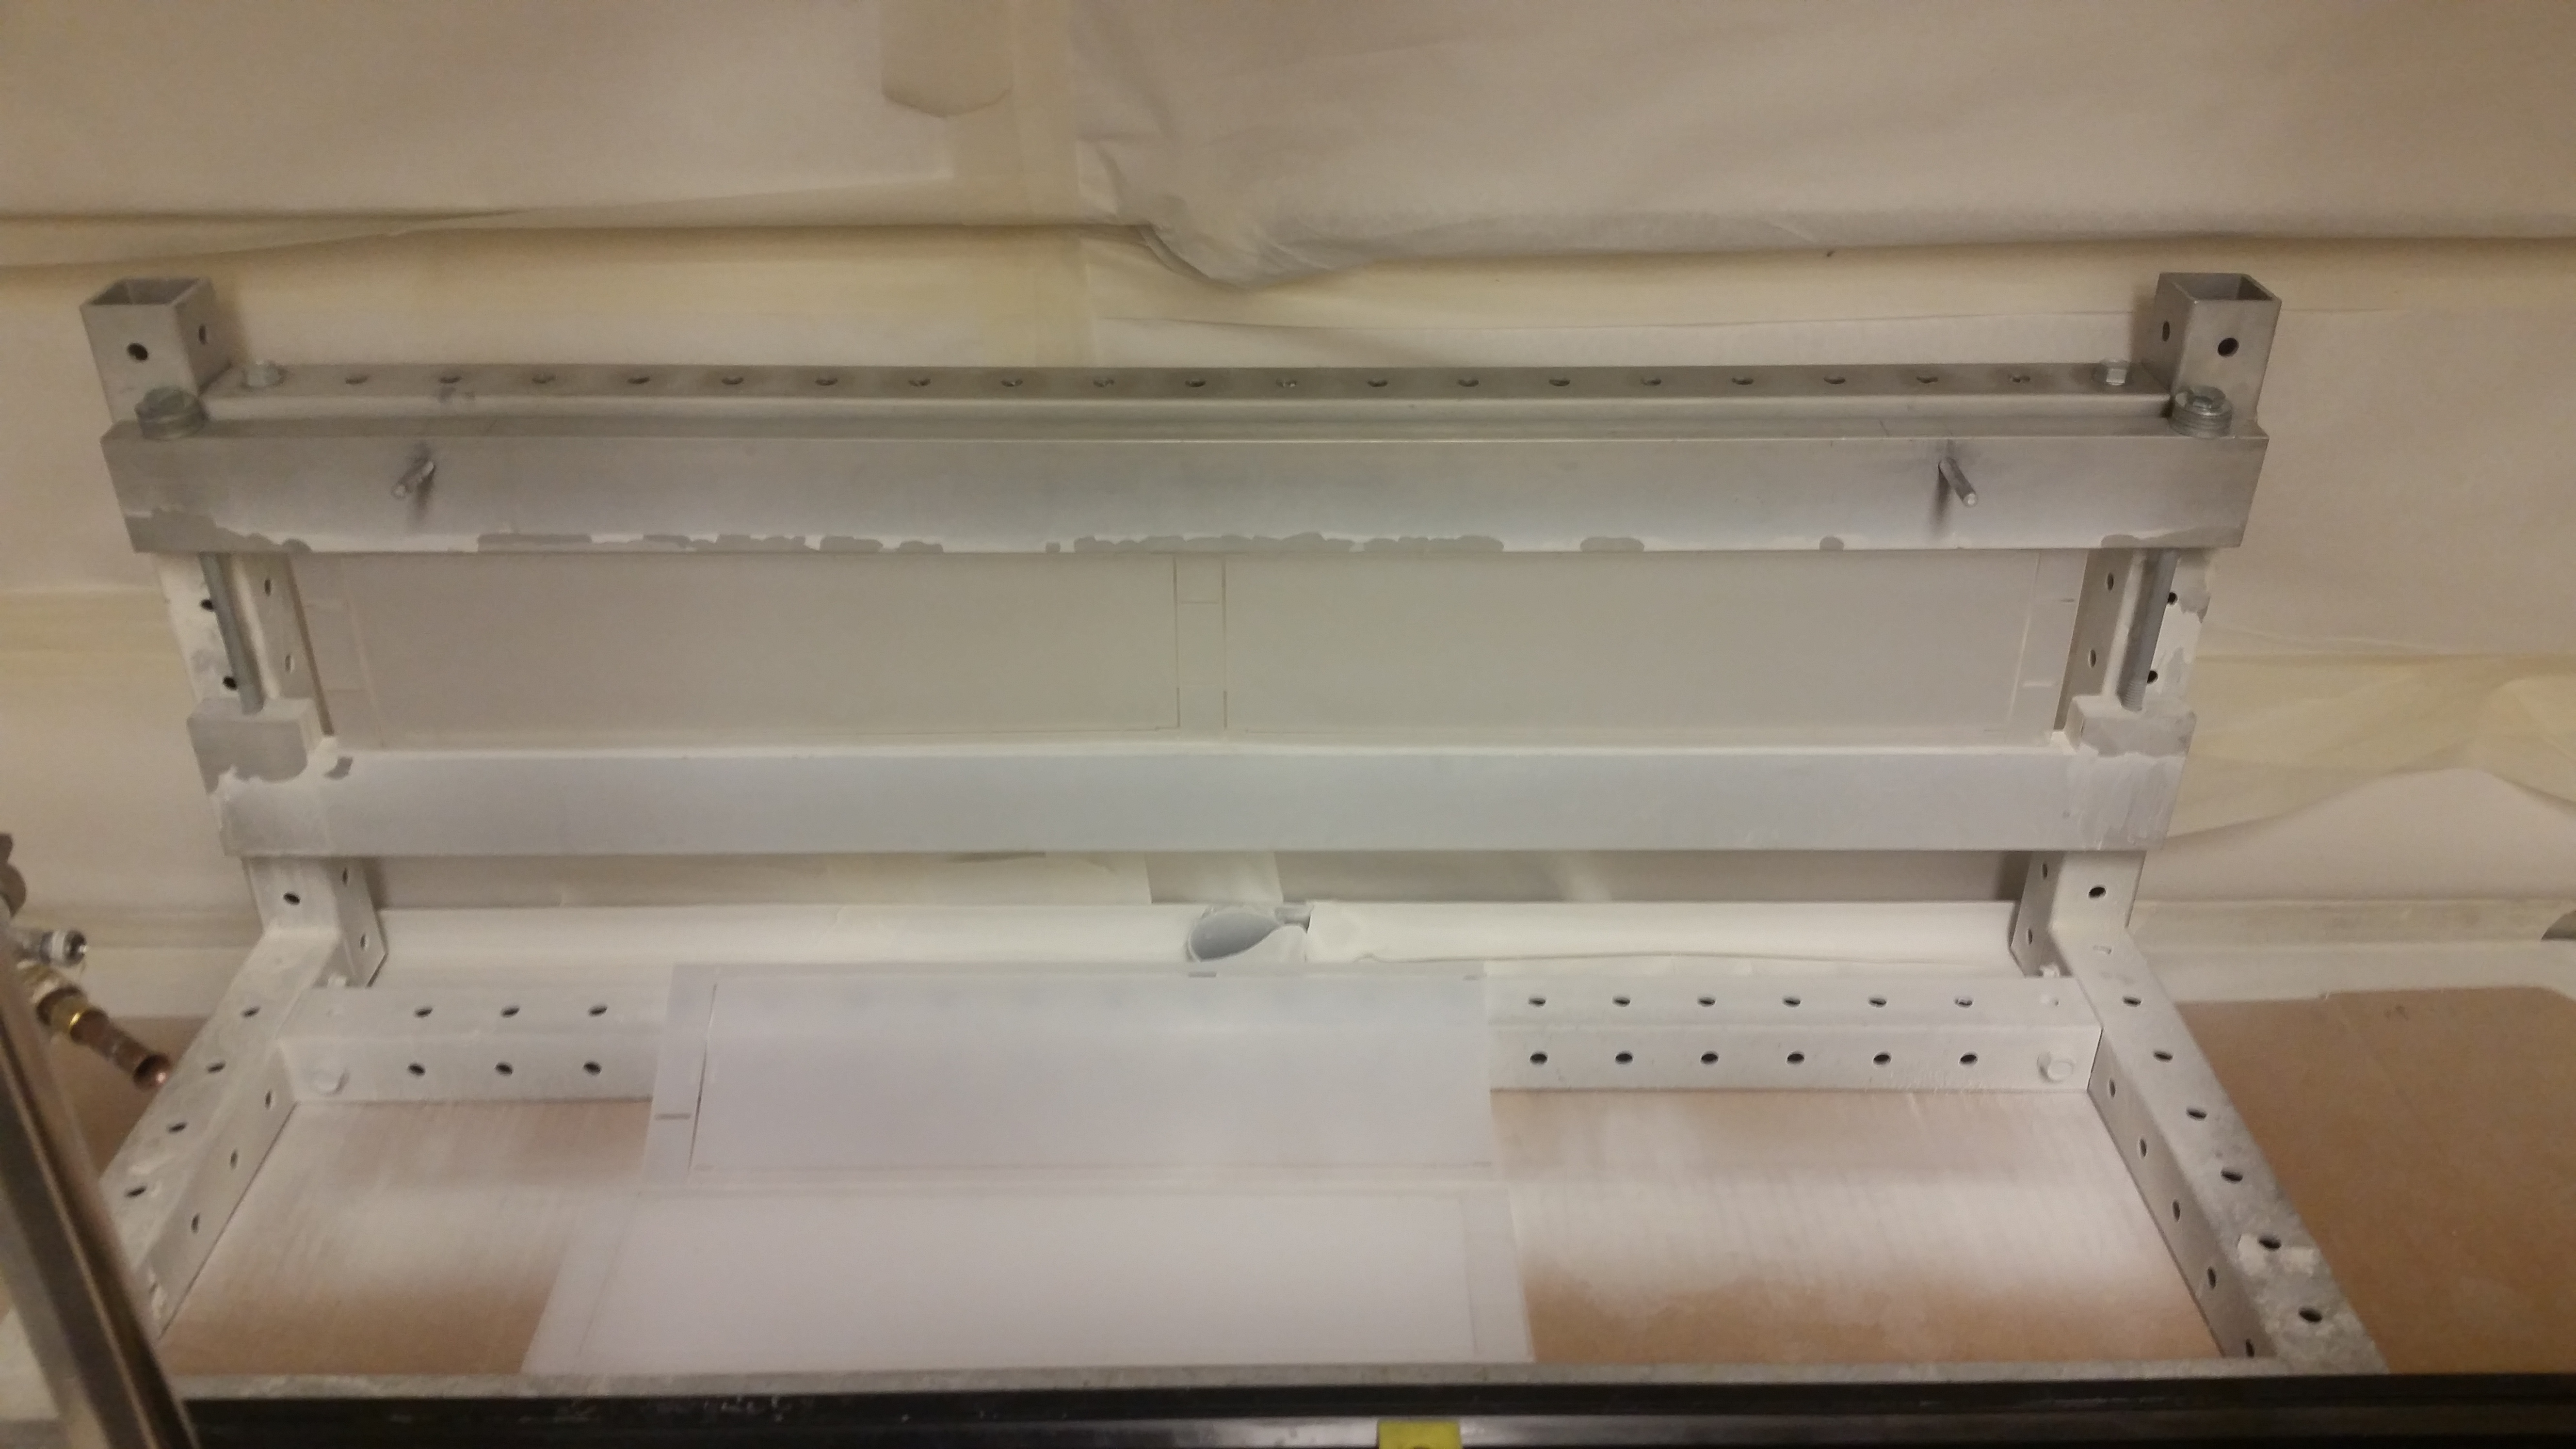
\includegraphics[width=0.9\columnwidth]{DoubleShiftLG-SprayedPlates.jpg}
  \caption{TPB-coated acrylic plates after spraying at Indiana University 
during fabrication of parts for ProtoDUNE-SP.}\label{fig:DoubleShiftLG-SprayedPlates}
  \end{center}
\end{figure}

\paragraph*{QA of the WLS Plates}

VUV conversion performance measured for neighboring samples from the 
acrylic plate template using a vacuum-ultraviolet monochromator.

\paragraph*{Receipt and QA of the Light Guides}

EJ-280 light guides fabricated by Eljen Technologies. Received and scanned in a 
long dark-box using a blue LED~(Fig.~\ref{fig:DoubleShiftLG-EJ280}).
 Measure conversion and transmission to the light guide ends to test attenuation. 
Direct transmission through the light guide to confirm uniformity. 
Attenuation length in liquid argon shorter than in air, but long attenuation in 
air has been shown to correspond to long attenuation in liquid argon.

\begin{figure}[ht]
  \begin{center}
 % 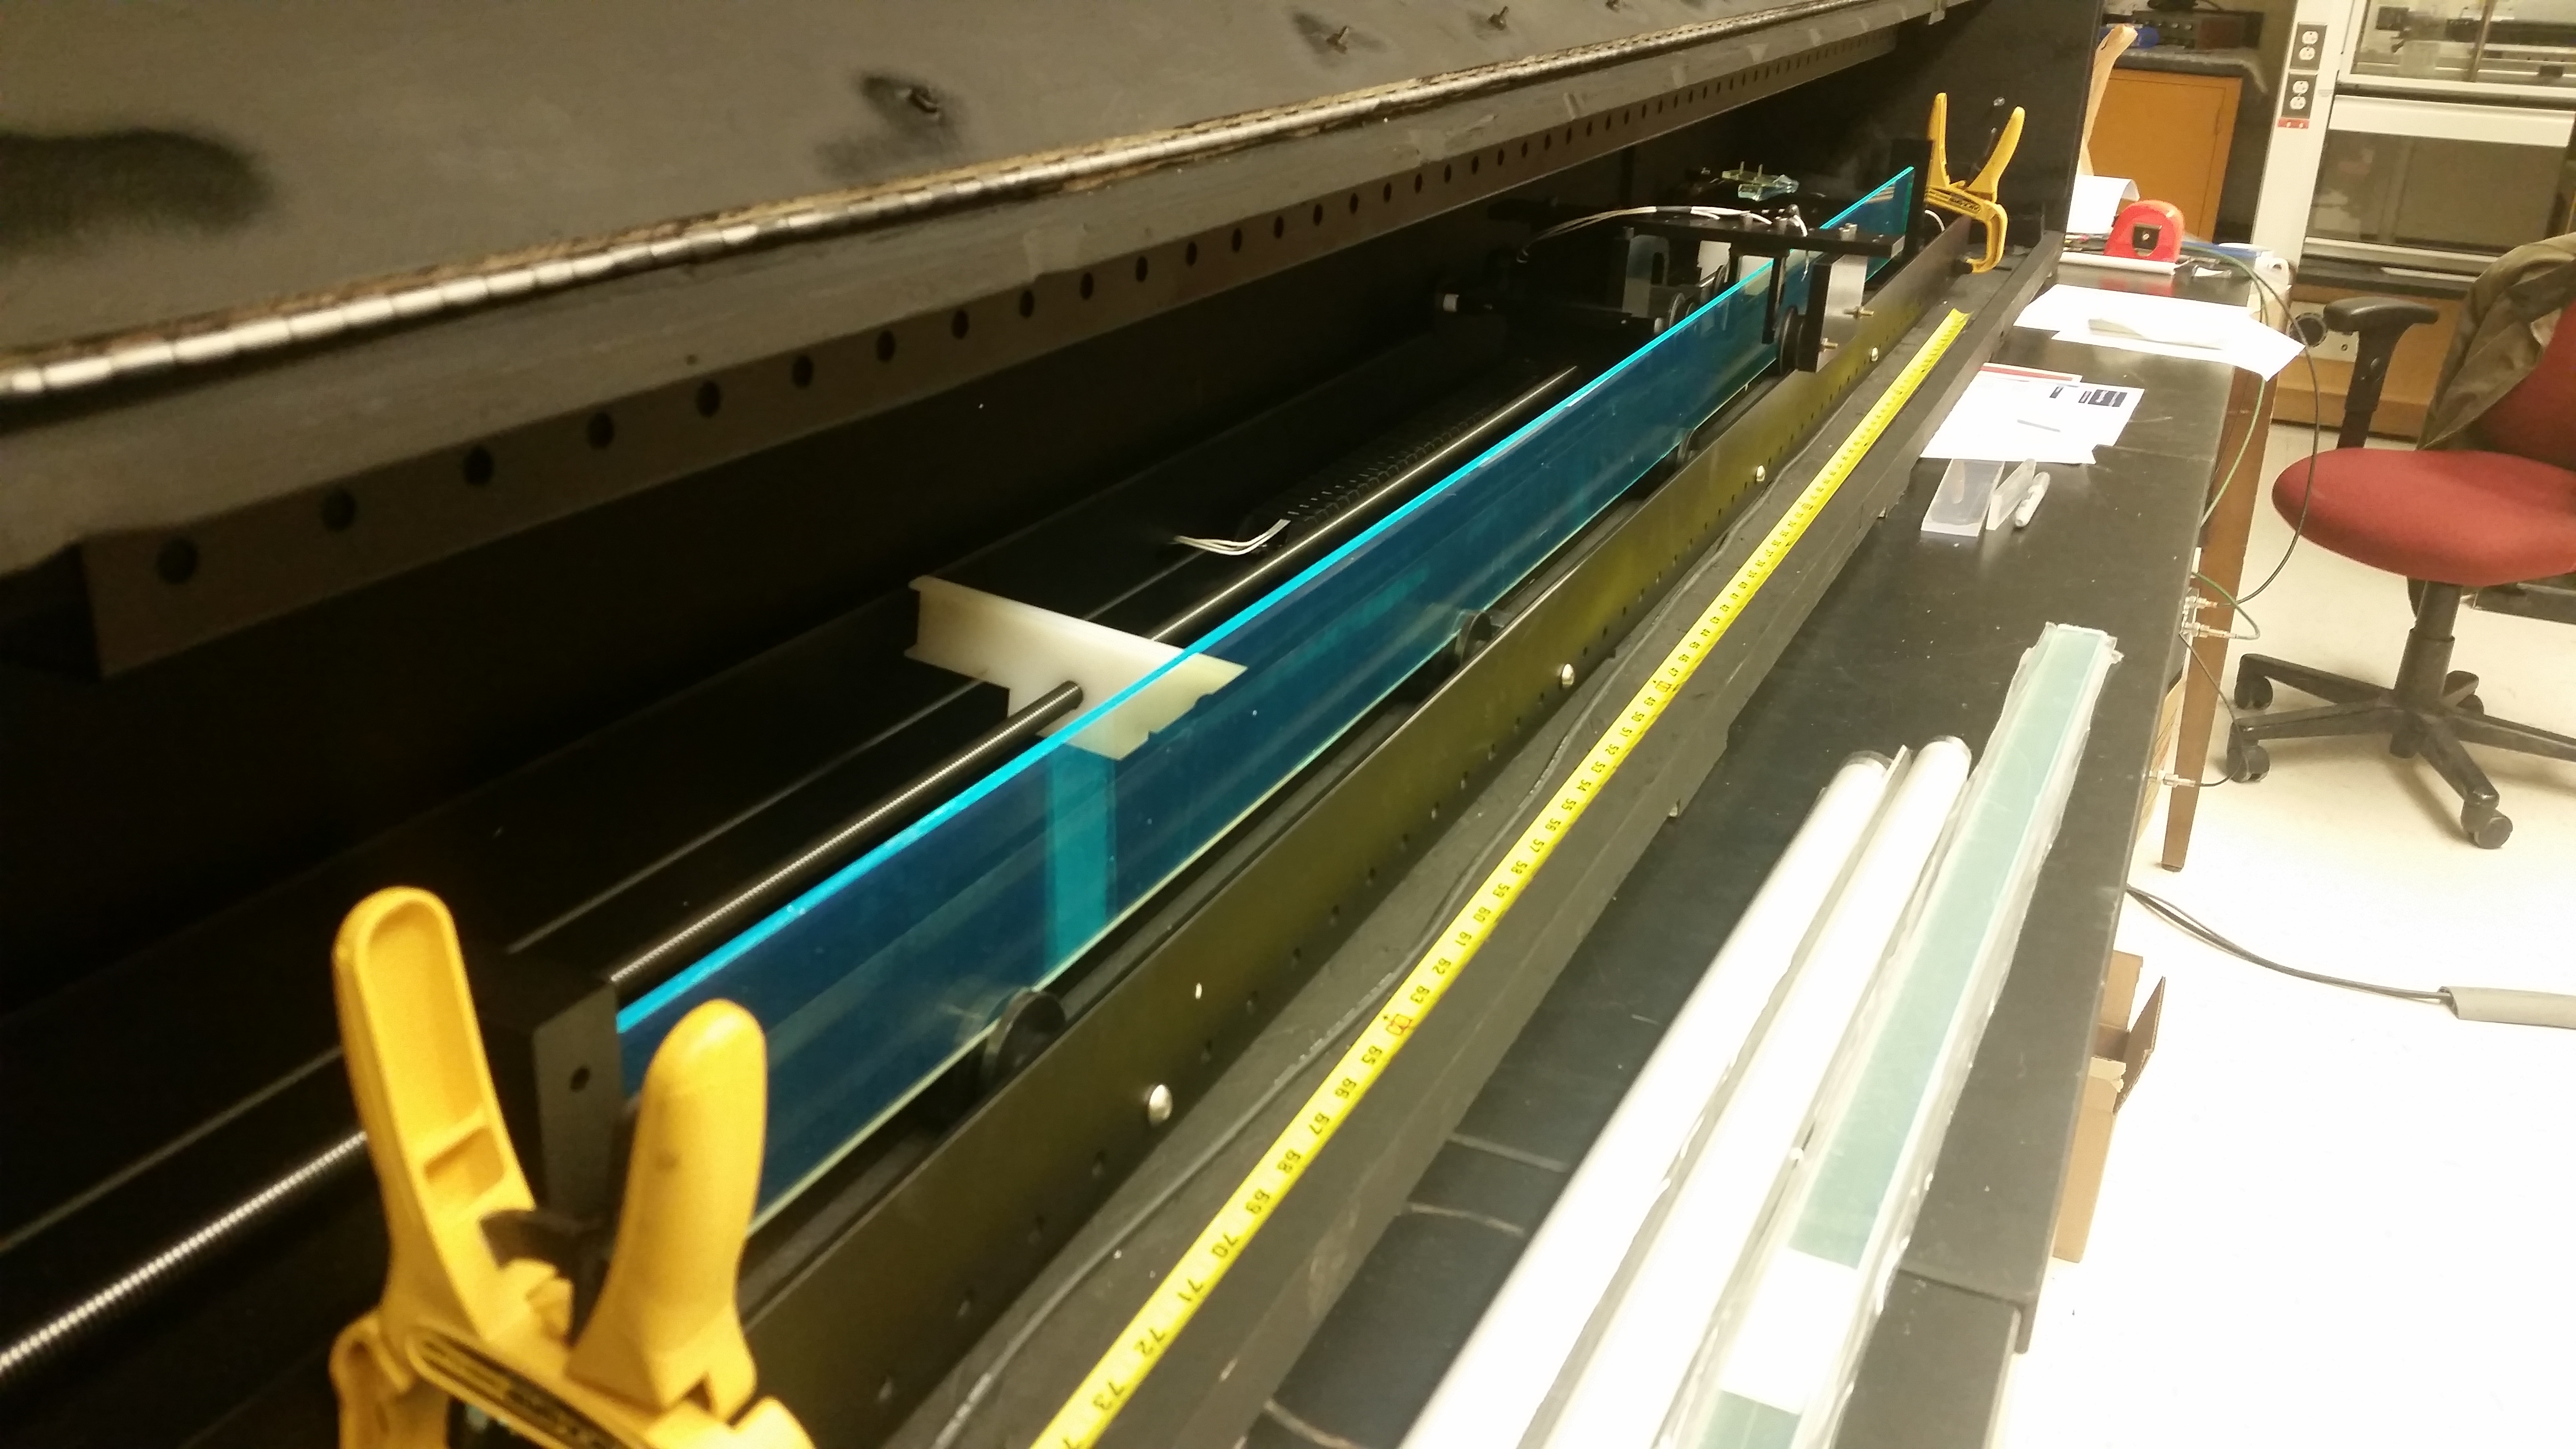
\includegraphics[width=0.9\columnwidth]{DoubleShiftLG-EJ280.jpg}
  \caption{EJ-280 light guide within darkbox for attenuation scan QA at 
Indiana University (prepared for ProtoDUNE-SP).}\label{fig:DoubleShiftLG-EJ280}
  \end{center}
\end{figure}

\paragraph*{Assembly of the Double-shift Light Guide Module}

Parts are shipped to the assembly point where the EJ-280 light guide is mounted 
into the module frame and the WLS plates are attached.

\begin{figure}[ht]
  \begin{center}
 % 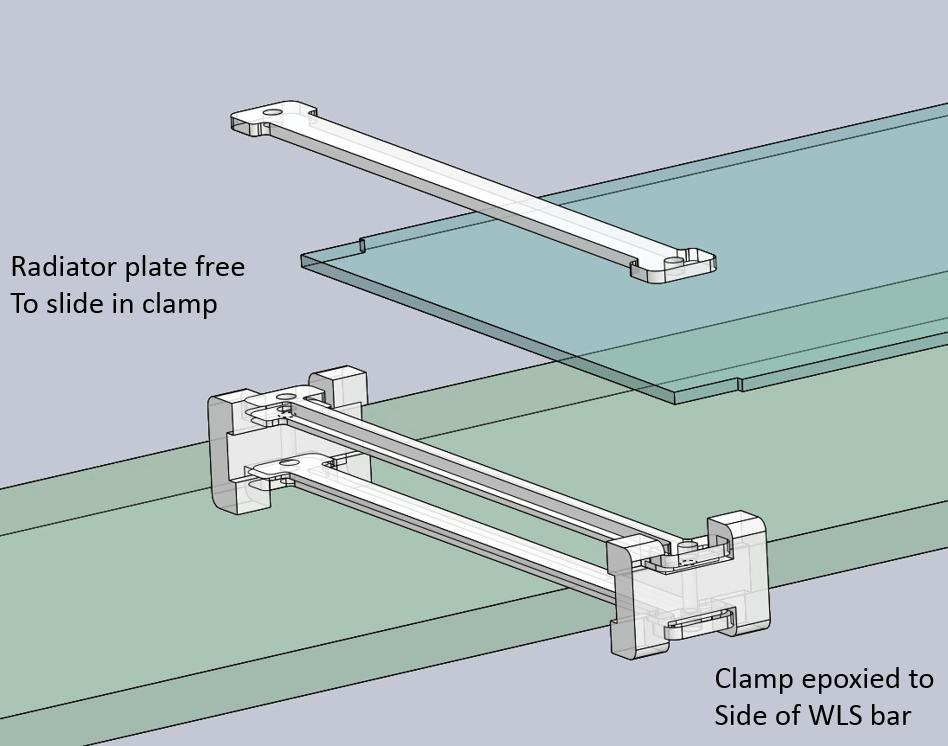
\includegraphics[width=0.9\columnwidth]{DoubleShiftLG-PlateMounting.jpg}
  \caption{Mounting of the WLS plates to the EJ-280 bar.}\label{fig:DoubleShiftLG-PlateMounting}
  \end{center}
\end{figure}


\subsubsection{ARAPUCA (2 pages)}
\label{ssec:fdsp-pd-pc-prod-arapuca}



%%%%%%%%%%%%%%%%%%%%%%%%%%%%%%%%%%
\subsection{Light Concentrators}
\label{sec:fdsp-pd-assy-lc}
\fixme{\color{blue} Content:  (1 page) - Cavanna}
	
\section{PD Production and Assembly: Light Concentrator}
In the current baseline layout, the photosensitive area of the PD system is limited to about 12.5\% of the area of the anode plane - delimiting one side of the LArTPC volume. 
Only a small fraction of the VUV direct light emitted in ionization events is thus intercepted by the photosensitive area, and this fraction also 
 quickly reduces at increasing distance of the event from the anode plane. \\
Methods to increase the amount of light collected by the PDS are being considered, for example by covering the opposite cathode plane with wls-coated reflector foils so that a good fraction of the VUV light is shifted into the Visible, reflected back toward the Anode plane and eventually intercepted by the PDS, if sensitive to this wavelength.

Further increase in light collection, both for the VUV and the reflected Vis component, can be achieved by implementing large area reflective surfaces 
at the anode plane (e.g. in the large open areas between PD bars inside the APA frames) acting as light concentrators toward the smaller photosensitive surfaces.  
This conceptual solution is suggested from the widely diffused implementation of Winston Cones for enhancing light collection in large volume liquid detectors. 
The PD bar geometry of the photosensitive area inside the thin APA frames and the related mechanical constraints impose rather severe limitations 
on the design - cone depth and entrance$/$exit apertures ratio - of the light concentrating surfaces. The installation of the reflective surfaces inside the APA frame would necessarily be made before wire winding. 
Ongoing studies are expected to demonstrate the feasibility of the solution and move the conceptual scheme into a technical design. MC simulations will determine the efficiency of the light concentrator. 




%%%%%%%%%%%%%%%%%%%%%%%%%%%%%%%%%%
\subsection{PD Mounting in APA Frames}
\label{sec:fdsp-pd-assy-frames}
\fixme{\color{blue} Content:   (2 pages) - Warner}

\subsubsection{APA Frame Mounting Structure and Module Fixing}	
Photon detector (PD) modules are inserted into the APA frames through ten slots 
(five on each side of the APA frame) and are supported in place inside the frame in 
stainless steel guide channels.  The slot dimensions for the ProtoDUNE APA frames 
were 108.0mm X 19.2mm wide (See fig. 1).  The guide channels are pre-positioned into 
the APA frame prior to applying the wire shielding mesh to the APA frames, and are
not accessible following wire wrapping.

\fixme{Insert Dave's PD Mounting rails in APA frame mpicture}

Following insertion, the PD modules are fixed in place in the APA frame using
 two stainless steel captive screws, as shown in figure 2.

\fixme{Insert Dave's PD Mounting screws mpicture}

\paragraph{Cryogenic thermal contraction}

Bar-style PD modules are structurally composed of primarily polycarbonate and 
acrylic, which have significantly different shrinkage factors compared to the 
stainless steel APA and PD support frames (see table 1).

\fixme{format table better?}

\begin{table}[h!]
\label{tbl:fdsfpdshrink}
\begin{center}
\caption{Shrinkage of Photon Detector Materials}
\begin{tabular}{|c|c|}
\hline
\textbf{Material Shrinkage Factor (m/m)} & \textbf{$206^{\circ}C$ Drop}\\
\hline
Stainless Steel (304) & $2.7*10^{-3}$\\
FR-4 G-10 (In-plane) & $2.1*10^{-3}$\\
Polystyrene (Average) & $1.5*10^{-2}$\\
Acrylic and Polycarbonate (Average) & $1.4*10^{-2}$\\
\hline
\end{tabular}
\end{center}
\end{table}

These differences in thermal expansion (or contraction in this case) were 
important to keep in mind during design of the PD module supports.  
Mitigation for these varying contractions are detailed in table 2:

\fixme{ Needs better table formatting? }

\begin{table}[h!]
\label{tbl:fdsfpdshrinkeffects}
\begin{center}
\caption{Relative Shrinkage of PD components and APA frame, and mitigations}
\begin{tabular}{|p{0.25\textwidth}|p{0.25\textwidth}|p{0.4\textwidth}}
\hline
\textbf{Interface} & \textbf{Relative shrinkage} & \textbf{Mitigation} \\
\hline
PD Length to APA width & PD shrinks 25.7mm Relative to APA frame & PD affixed only at one end of APA frame, free to contract at other end \\
\hline
Width of PD in APA Slot & PD shrinks 1.2mm relative to slot width & Photon detector not constrained in C-channels. C channels and tolerances designed to contain module across thermal contraction range \\
\hline
Width of SiPM mount board (\it(Hover board)) to stainless steel frame & Stainless frame shrinks 0.06mm more than PCB & Diameter of shoulder screws and FR-4 board clearance holes selected to allow for motion \\
\hline
Width of SiPM mount board relative to polycarbonate mount block & Polycarbonate block shrinks 1mm more than PCB & Allowed for in clearance holes in SiPM mount board \\
\hline
\end{tabular}
\end{center}
\end{table}


\paragraph{PD Mount Frame Deformation under static PD load}

FEA modeling of the PD support structure was conducted to study static deflection 
prior to building prototypes.  Modeling was conducted in both the vertical
 orientation (APA upright, as installed in cryostat) and also flat.  
Basic assumptions used were fully-supported fixed end conditions for the rails, 
uniform loading of 3X PD mass (5 kg) along rails.  
Prototype testing confirmed these calculations.

\fixme{Insert Dave's 4 deflection pictures here}


\fixme{Same for bars and ARAPUCAs}

%%%%%%%%%%%%%%%%%%%%%%%%%%%%%%%%%%
\subsection{Photosensor Modules}
\label{sec:fdsp-pd-assy-psm}
\fixme{\color{blue} Content:  (1 page) - Zutshi}

The Silicon Photomultiplier analog signal will be ganged on the detector inside the
LAr volume. Passive and active ganging schemes are under consideration. Some passive
ganging (sensors put in parallel) schemes have been examined and are being installed inside
proto-DUNE (see Fig. yyy). The key point for parallel passive ganging in terms of 
maintaining signal-to-noise as devices are ganged together is the terminal capacitance of the 
sensors. This characteristics can therefore play an important in device selection or on
the flip side in determining the maximum ganging possible. In this scheme the 
ganged analog signals are then brought out via long cables (~25 m) for digitization outside
the cryostat. This is currently being done in proto-DUNE using teflon ethernet CAT6 cables.

An interesting alternative option that may provide more flexibility in terms of the level of
photosensor ganging possible and also obviate the need for carrying analog signals of long cables
is the so-called active ganging option where the amplifiers and ADCs sit on the board carrying 
the photosensors inside the LAr volume. This option however brings, in all the reliability and long-term
stability issues related to cold electronics into play. While active ganging prototypes are under study 
the design cannot be considered to be at a mature stage at this point and schedule and technical
considerations may influence how far this promising option can be pursued.

In any case, the SiPMs will need to be surface-mounted on a PCB that can mate efficiently with the photon
collector options. proto-DUNE will provide a wealth of operational experience and information on
such a design with atleast a passive ganging board. It is already clear, however, that some R$\&$D is needed 
in optimizing the connectors to be used to couple the cable to the board and understanding the 
mechanical stresses involved in the SiPM-PCB-Connector system (with a varying CTEs) as it
is cooled (or cycled) to cryogenic temperatures.



\fixme{Just cold boards?}

%%%%%%%%%%%%%%%%%%%%%%%%%%%%%%%%%%
%\subsection{(Common Tooling} -- Probably not worth bothering about, except for QA/QC scanners, etc.
%\label{sec:fdsp-pd-assy-ct}
%\fixme{\color{blue} Content:  Warner}
%\fixme{Is there common tooling or is described separately in the PC section?}

%%%%%%%%%%%%%%%%%%%%%%%%%%%%%%%%%%
\subsection{Assembly Procedures}
\label{sec:fdsp-pd-assy-ap}
\fixme{\color{blue} Content: Cavanna/Whittington/Machado}

PC assembly modules (ready for APA installation).

\fixme{Can we have a single section that describes how the bars and/or ARAPUCA are assembled into PC modules or do we need a separate subsub(!)section for each?}

\subsubsection{Dip-Coated Light Guide Modules (2 pages)}
\label{ssec:fdsp-pd-pc-assy-bar1}

\subsubsection{Double-Shift Light Guide Modules (2 pages)}
\label{ssec:fdsp-pd-pc-assy-bar2}

\subsubsection{ARAPUCA Modules (2 pages)}
\label{ssec:fdsp-pd-pc-assy-arapuca}


%%%%%%%%%%%%%%%%%%%%%%%%%%%%%%%%%%
\subsection{Electronics}
\label{sec:fdsp-pd-assy-pde}
\fixme{\color{blue} Content: (2 pages) Moreno/Franchi/Djuric}


\begin{itemize}
\item Components
\item Boards
\item Cable plant
\end{itemize}

%%%%%%%%%%%%%%%%%%%%%%%%%%%%%%%%%%
\subsection{QA}
\label{sec:fdsp-pd-assy-qa}
\fixme{\color{blue} Content:  (2 pages) - Warner}

\begin{itemize}
\item Sub-assemblies- same for all modules.
\item Completed modules- largely same for different option, at least for TP.
\end{itemize}


%%%%%%%%%%%%%%%%%%%%%%%%%%%%%%%%%%%%%%%%%%%%%%%%%%%%%%%%%%%%%%%%%%%%
\section{System Interfaces}
\label{sec:fdsp-pd-intfc}
\fixme{\color{blue} Content: Kemp}
\fixme{(Length: TDR=10 pages, TP=2 pages)}

\fixme{Include an image of each interface in appropriate section.}


%%%%%%%%%%%%%%%%%%%%%%%%%%%%%%%%%%%
\subsection{Anode Plane Assembly}
\label{sec:fdsp-pd-intfc-apa}

The Technical Proposal may include any suggestions or requests from the Photon Detector Consortium
for changes to the APA design. Any such changes need to be proposed as early as possible to ensure
consideration within the APA Consortium's schedule. Some examples include:
\begin{itemize}
\item Additional light collector bays
\item Alternate outer APA designs
\end{itemize}

%%%%%%%%%%%%%%%%%%%%%%%%%%%%%%%%%%%
\subsection{Feedthroughs}
\label{sec:fdsp-pd-intfc-feed}

%%%%%%%%%%%%%%%%%%%%%%%%%%%%%%%%%%%
\subsection{Electronics}
\label{sec:fdsp-pd-intfc-feed}

%%%%%%%%%%%%%%%%%%%%%%%%%%%%%%%%%%%
\subsection{Light Enhancement}
\label{sec:fdsp-pd-intfc-le}

%%%%%%%%%%%%%%%%%%%%%%%%%%%%%%%%%%%
\subsection{DAQ}
\label{sec:fdsp-pd-intfc-daq}

%%%%%%%%%%%%%%%%%%%%%%%%%%%%%%%%%%%
\subsection{Calibration/monitoring}
\label{sec:fdsp-pd-intfc-calib}



%%%%%%%%%%%%%%%%%%%%%%%%%%%%%%%%%%%%%%%%%%%%%%%%%%%%%%%%%%%%%%%%%%%%
\section{Installation, Integration and Commissioning}
\label{sec:fdsp-pd-install}
\fixme{\color{blue} Content: Kemp}
\fixme{(Length: TDR=30 pages, TP=6 pages)}

%%%%%%%%%%%%%%%%%%%%%%%%%%%%%%%%%%%%
\subsection{Transport and Handling (1 page)}
\label{sec:fdsp-pd-install-transport}


%%%%%%%%%%%%%%%%%%%%%%%%%%%%%%%%%%%
\subsection{Integration with APA  (2 pages)}
\label{sec:fdsp-pd-install-pd-apa}

%%%%%%%%%%%%%%%%%%%%%%%%%%%%%%%%%%%
\subsection{Installation into cryostat/cabling  (1 pages)}
\label{sec:fdsp-pd-install-pd-cryo}

%%%%%%%%%%%%%%%%%%%%%%%%%%%%%%%%%%%
\subsection{Calibration/Monitoring  (1 pages)}
\label{sec:fdsp-pd-install-calib}


%%%%%%%%%%%%%%%%%%%%%%%%%%%%%%%%%%%%%%%%%%%%%%%%%%%%%%%%%%%%%%%%%%%%
\section{Quality Control}
\label{sec:fdsp-pd-qc}
\fixme{\color{blue} Content: Warner}
\fixme{(Length: TDR=10 pages, TP=2 pages)}


%%%%%%%%%%%%%%%%%%%%%%%%%%%%%%%%%%%%
\subsection{Production and Assembly (Local)}
\label{sec:fdsp-pd-qc-local}


%%%%%%%%%%%%%%%%%%%%%%%%%%%%%%%%%%%
\subsection{Post-factory Installation (Remote)}
\label{sec:fdsp-pd-qc-remote}


%%%%%%%%%%%%%%%%%%%%%%%%%%%%%%%%%%%%%%%%%%%%%%%%%%%%%%%%%%%%%%%%%%%%
\section{Safety}
\label{sec:fdsp-pd-safety}
\fixme{\color{blue} Content: Warner}
\fixme{(Length: TDR=5 pages, TP=1 pages)}

%%%%%%%%%%%%%%%%%%%%%%%%%%%%%%%%%%%
% add subsections and labels if needed \subsection{}
%\subsection{}
%\label{sec:fdsp-pd-safety}



%%%%%%%%%%%%%%%%%%%%%%%%%%%%%%%%%%%%%%%%%%%%%%%%%%%%%%%%%%%%%%%%%%%%
\section{Organization}
\label{sec:fdsp-pd-org}
\fixme{\color{blue} Content: Segreto/Warner/Mualem}
\fixme{(Length: TDR=20 pages, TP=4 pages)}

%%%%%%%%%%%%%%%%%%%%%%%%%%%%%%%%%%%
\subsection{Single-Phase Photon Detection System Consortium Organization}
\label{sec:fdsp-pd-org-consortium}
\fixme{\color{blue} Content: Segreto}


%%%%%%%%%%%%%%%%%%%%%%%%%%%%%%%%%%
\subsection{Planning Assumptions}
\label{sec:fdsp-pd-org-assmp}
\fixme{\color{blue} Content: Segreto/Warner}


%%%%%%%%%%%%%%%%%%%%%%%%%%%%%%%%%%%
\subsection{WBS and Responsibilities}
\label{sec:fdsp-pd-org-wbs}
\fixme{\color{blue} Content: Warner/Mualem}

%%%%%%%%%%%%%%%%%%%%%%%%%%%%%%%%%%
\subsection{High-level Cost and Schedule}
\label{sec:fdsp-pd-org-cs}
\fixme{\color{blue} Content: Warner/Mualem}













